% Paquets généraux
\documentclass[a4paper,12pt,titlepage]{article}
\usepackage[T1]{fontenc}
\usepackage[utf8]{inputenc}
\usepackage[french]{babel}
\usepackage[gen]{eurosym}
%\usepackage[dvips]{graphicx}
\usepackage{fancyhdr}
\usepackage{pdfpages} 
\usepackage{multido}
\usepackage{hyperref}
%\usepackage{textcomp}
%\usepackage{aeguill}
\usepackage{schemabloc}
\usepackage[bitstream-charter]{mathdesign}
\usepackage{minted}

\newcommand{\id}{71}
\newcommand{\nom}{Théorie des mécanismes}
\newcommand{\sequence}{04}
\newcommand{\nomsequence}{Liaisons entre les solides}
\newcommand{\num}{02}
\newcommand{\type}{KH}
\newcommand{\descrip}{Liaisons équivalentes, hyperstatisme, liaisons en série et en parallèle, théorie des graphes}
\newcommand{\competences}{B2-12: Proposer une modélisation des liaisons avec leurs caractéristiques géométriques. \\ &  B2-13: Proposer un modèle cinématique paramétré à partir d'un système réel, d'une maquette numérique ou d'u \\ &  B2-17: Simplifier un modèle de mécanisme. \\ &  B2-18: Modifier un modèle pour le rendre isostatique. \\ &  C1-04: Proposer une démarche permettant d'obtenir une loi entrée-sortie géométrique.  \\ &  C2-05: Caractériser le mouvement d'un repère par rapport à un autre repère. \\ &  C2-06: Déterminer les relations entre les grandeurs géométriques ou cinématiques. }
\newcommand{\nbcomp}{7}
\newcommand{\systemes}{}
\newcommand{\systemesnum}{}
\newcommand{\systemessansaccent}{}
\newcommand{\ilot}{2}
\newcommand{\ilotstr}{02}
\newcommand{\dossierilot}{\detokenize{Ilot_02 }}


\newcommand{\auteurun}{Renaud Costadoat}
\newcommand{\auteurdeux}{Françoise Puig}
\newcommand{\institute}{Lycée Dorian}


\usepackage{color}
\usepackage{xcolor}
\usepackage{colortbl}
\usepackage{helvet}
\usepackage[frenchmath]{newtxsf} % for sans serif symbols
\renewcommand{\familydefault}{\sfdefault}
%\usepackage{amsfonts}
%\usepackage{amsmath}
%\usepackage{lmodern}
\usepackage{mathastext}
%\usepackage{xspace}
\usepackage{varioref}
\usepackage{tabularx}
%\usepackage{floatflt}
\usepackage{graphics}
\usepackage{wrapfig}
\usepackage{textcomp}
\usepackage{tikz}
\usepackage{wrapfig}
\usepackage{gensymb}
\usepackage[european]{circuitikz}
\usetikzlibrary{babel}
\usepackage{ifthen}
\usepackage{cancel}
\usepackage{etoolbox}
\usepackage{multirow}
%\usepackage{boxedminipage}
\definecolor{gris25}{gray}{0.75}
\definecolor{bleu}{RGB}{18,33,98}
\definecolor{bleuf}{RGB}{42,94,171}
\definecolor{bleuc}{RGB}{231,239,247}
\definecolor{rougef}{RGB}{185,18,27}
\definecolor{rougec}{RGB}{255,188,204}%255,230,231
\definecolor{vertf}{RGB}{103,126,82}
\definecolor{vertc}{RGB}{220,255,191}
\definecolor{forestgreen}{rgb}{0.13,0.54,0.13}
\definecolor{blcr}{rgb}{0.59,0.69,0.84}
\definecolor{blfr}{rgb}{0.32,0.51,0.75}
\definecolor{orfr}{rgb}{0.90,0.42,0.15}
\definecolor{orcr}{rgb}{0.90,0.65,0.50}
\definecolor{orangef}{rgb}{0.659,0.269,0.072}
\definecolor{orange}{rgb}{0.58,0.35,0.063}
\definecolor{orangec}{rgb}{0.43,0.32,0.25}
\definecolor{rcorrect}{rgb}{0.6,0,0}
\definecolor{sequence}{rgb}{0.75,0.75,0.75}
\definecolor{competences}{rgb}{0.61,0.73,0.35}
\definecolor{grisf}{HTML}{222222}
\definecolor{grisc}{HTML}{636363}
\definecolor{normal}{HTML}{4087c4}
\definecolor{info}{HTML}{5bc0de}
\definecolor{success}{RGB}{92,184,92}
\definecolor{warning}{RGB}{240,173,78}
\definecolor{danger}{RGB}{217,83,79}
\hypersetup{                    % parametrage des hyperliens
    colorlinks=true,                % colorise les liens
    breaklinks=true,                % permet les retours à la ligne pour les liens trop longs
    urlcolor= blfr,                 % couleur des hyperliens
    linkcolor= orange,                % couleur des liens internes aux documents (index, figures, tableaux, equations,...)
    citecolor= forestgreen                % couleur des liens vers les references bibliographiques
    }

% Mise en page
\pagestyle{fancy}

\setlength{\hoffset}{-18pt}

\setlength{\oddsidemargin}{0pt} 	% Marge gauche sur pages impaires
\setlength{\evensidemargin}{0pt} 	% Marge gauche sur pages paires
\setlength{\marginparwidth}{00pt} 	% Largeur de note dans la marge
\setlength{\headwidth}{481pt} 	 	% Largeur de la zone de tête (17cm)
\setlength{\textwidth}{481pt} 	 	% Largeur de la zone de texte (17cm)
\setlength{\voffset}{-18pt} 		% Bon pour DOS
\setlength{\marginparsep}{7pt}	 	% Séparation de la marge
\setlength{\topmargin}{-30pt} 		% Pas de marge en haut
\setlength{\headheight}{35pt} 		% Haut de page
\setlength{\headsep}{20pt} 		% Entre le haut de page et le texte
\setlength{\footskip}{30pt} 		% Bas de page + séparation
\setlength{\textheight}{700pt} 		% Hauteur de l'icone zone de texte (25cm)
\setlength\fboxrule{1 pt}
\renewcommand{\baselinestretch}{1}
\setcounter{tocdepth}{1}
\newcommand{\cadre}[2]
{\fbox{
  \begin{minipage}{#1\linewidth}
   \begin{center}
    #2\\
   \end{center}
  \end{minipage}
 }
}

\newcounter{num_quest} \setcounter{num_quest}{0}
\newcounter{num_rep} \setcounter{num_rep}{0}
\newcounter{num_cor} \setcounter{num_cor}{0}

\newcommand{\question}[1]{\refstepcounter{num_quest}\par
~\ \\ \parbox[t][][t]{0.15\linewidth}{\textbf{Question \arabic{num_quest}}}\parbox[t][][t]{0.93\linewidth}{#1}\par
}


\newcommand{\reponse}[1]
{\refstepcounter{num_rep}
\noindent
\rule{\linewidth}{.5pt}
\textbf{Question \arabic{num_rep}:}
\multido{\i=1+1}{#1}{~\ \\}
}

\newcommand{\cor}
{\refstepcounter{num_cor}
\noindent
\rule{\linewidth}{.5pt}
\textbf{Question \arabic{num_cor}:} \\
}

\newcommand{\titre}[1]
{\begin{center}
\cadre{0.8}{\huge #1} 
\end{center}
}


% En tête et pied de page
\fancypagestyle{normal}{%
  \fancyhf{}
\lhead{\nom}
\rhead{
\includegraphics[width=2cm]{../../img/logo}\hspace{2pt}}
\ifdef{\auteurdeux}{\lfoot{\auteurun,\auteurdeux}}{\lfoot{\auteurun}}
\cfoot{Page \thepage}}

\fancypagestyle{correction}{%
  \fancyhf{}
  \lhead{\colorbox{danger}{\begin{minipage}{0.65\paperwidth} \textcolor{white}{\textbf{Correction}} \end{minipage}} }
  \rhead{
\includegraphics[width=2cm]{../../img/logo}}
  \ifdef{\auteurdeux}{\lfoot{\auteurun,\auteurdeux}}{\lfoot{\auteurun}}
  \rfoot{\colorbox{danger}{\begin{minipage}{0.5\paperwidth} \begin{flushright}\textcolor{white}{\textbf{Correction}}\end{flushright} \end{minipage}} }}

\renewcommand{\footrulewidth}{0.4pt}

\usepackage{eso-pic}
\newcommand{\BackgroundPic}{%
\put(0,0){%
\parbox[b][\paperheight]{\paperwidth}{%
\vfill
\begin{center}
\hspace{0.5cm}\vspace{0.5cm}

\includegraphics[width=\paperwidth,height=\paperheight,%
keepaspectratio]{../../img/fond3}%
\end{center}
\vfill
}}}

\newcommand{\BackgroundPicdeux}{%
\put(25,-30){%
\parbox[b][\paperheight]{\paperwidth}{%
\vfill
\begin{center}

\includegraphics[width=\paperwidth,height=\paperheight,%
keepaspectratio]{../../img/fond4}%
\end{center}
\vfill
}}}

\begin{document}

\pagestyle{empty}

\vspace*{-3\baselineskip}

\AddToShipoutPicture*{\BackgroundPic}

\ifdef{\auteurdeux}{\begin{tabular}{>{\columncolor{gray!00}}m{.3\linewidth} m{.3\linewidth} >{\columncolor{gray!00}}m{.3\linewidth}}
Séquence : \sequence &  \multirow{3}{*}{\hspace{1cm}
\includegraphics[height=1.5cm]{../../img/logo}} &  \begin{flushright} \multirow{4}{*}{\hspace{1cm}\includegraphics[height=4cm]{img/qrcode}}\end{flushright}\\
Document : \type\num \\
 \institute \\
 \auteurun\\
 \auteurdeux
\end{tabular}}{\begin{tabular}{>{\columncolor{gray!00}}m{.3\linewidth} m{.3\linewidth} >{\columncolor{gray!00}}m{.3\linewidth}}
Séquence : \sequence &  \multirow{3}{*}{\hspace{1cm}
\includegraphics[height=1.5cm]{../../img/logo}} &  \begin{flushright} \multirow{4}{*}{\hspace{1cm}\includegraphics[height=4cm]{img/qrcode}}\end{flushright}\\
Document : \type\num \\
 \institute \\
 \auteurun
\end{tabular}}

\vspace{1cm}

\ifdef{\prive}{\begin{center}\colorbox{danger}{\Huge{Avec Correction}}\end{center}}{}

\begin{center}\huge{\nom}\end{center}

\vspace{2cm}

\ifdef{\imagedeux}{\begin{minipage}{0.49\linewidth}}{}
\begin{center}\includegraphics[height=5cm]{/home/renaud/Documents/Renaud/GitHub/django_education/systemes/\imageun}\end{center}
\ifdef{\imagedeux}{\end{minipage}\hfill
\begin{minipage}{0.49\linewidth}
\begin{center}\includegraphics[height=5cm]{/home/renaud/Documents/Renaud/GitHub/django_education/systemes/\imagedeux}\end{center}
\end{minipage}}{}

\vspace{5cm}


\begin{tabular}{p{.15\linewidth} >{\columncolor{white}}p{.8\linewidth}}
    \rowcolor{gray!20}
    Référence & S\sequence\ - \type\num \\
    Compétences & \competences \\
 	\rowcolor{gray!20}
    Description & \descrip \\
    Système & \systemes
  \end{tabular}

\newpage

\AddToShipoutPicture{\BackgroundPicdeux}

\pagestyle{normal}

\section{Présentation du système}

\begin{figure}[ht!]
 \begin{minipage}{0.55\linewidth}
Le système étudié est une calculatrice de bureau utilisée pour des opérations financières ou comptables.

Le but de ce TP est de modéliser, de simuler et de valider deux solutions technologiques pour la réalisation d'un additionneur:
\begin{itemize}
 \item logique câblée (simulée sous Matlab/Simulink),
 \item logique programmée (simulée sous python)
\end{itemize}
 \end{minipage}
 \hfill
  \begin{minipage}{0.4\linewidth}
   \centering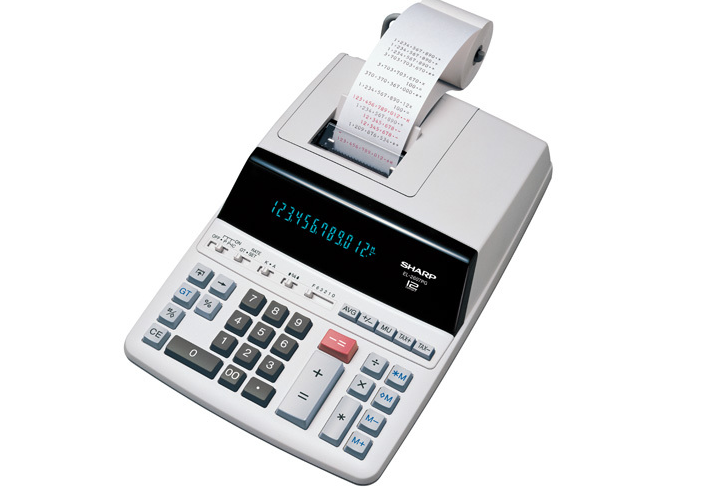
\includegraphics[width=0.7\linewidth]{img/calculatrice.png}
  \end{minipage}
\end{figure}

Des fichiers sont donnés afin de démarrer d'exercice:
\begin{itemize}
 \item Un fichier Simulink : \href{https://raw.githubusercontent.com/Costadoat/Sciences-Ingenieur/master/S07\%20Les\%20syst\%C3\%A8mes\%20\%C3\%A0\%20\%C3\%A9v\%C3\%A8nements\%20discrets/TP01\%20Fonctions\%20combinatoires/Ilot_01\%20Calculatrice\%20de\%20bureau/Code/Calculatrice\_vierge.slx}{Calculatrice vierge.slx},
 \item Un fichier Python : \href{https://raw.githubusercontent.com/Costadoat/Sciences-Ingenieur/master/S07\%20Les\%20syst\%C3\%A8mes\%20\%C3\%A0\%20\%C3\%A9v\%C3\%A8nements\%20discrets/TP01\%20Fonctions\%20combinatoires/Ilot_01\%20Calculatrice\%20de\%20bureau/Code/Calculatrice\_vierge.py}{Calculatrice vierge.py}.

\end{itemize}

\section{Additionner deux nombres de 1 bit}

\begin{minipage}{0.7\linewidth}
Nous allons tout d'abord réaliser un additionneur à 1 chiffre binaire. C'est un composant ayant deux entrées logiques (les deux chiffres binaires à additionner) notés $a_0$ et $b_0$.
\end{minipage}
\hfill
\begin{minipage}{0.28\linewidth}
 \centering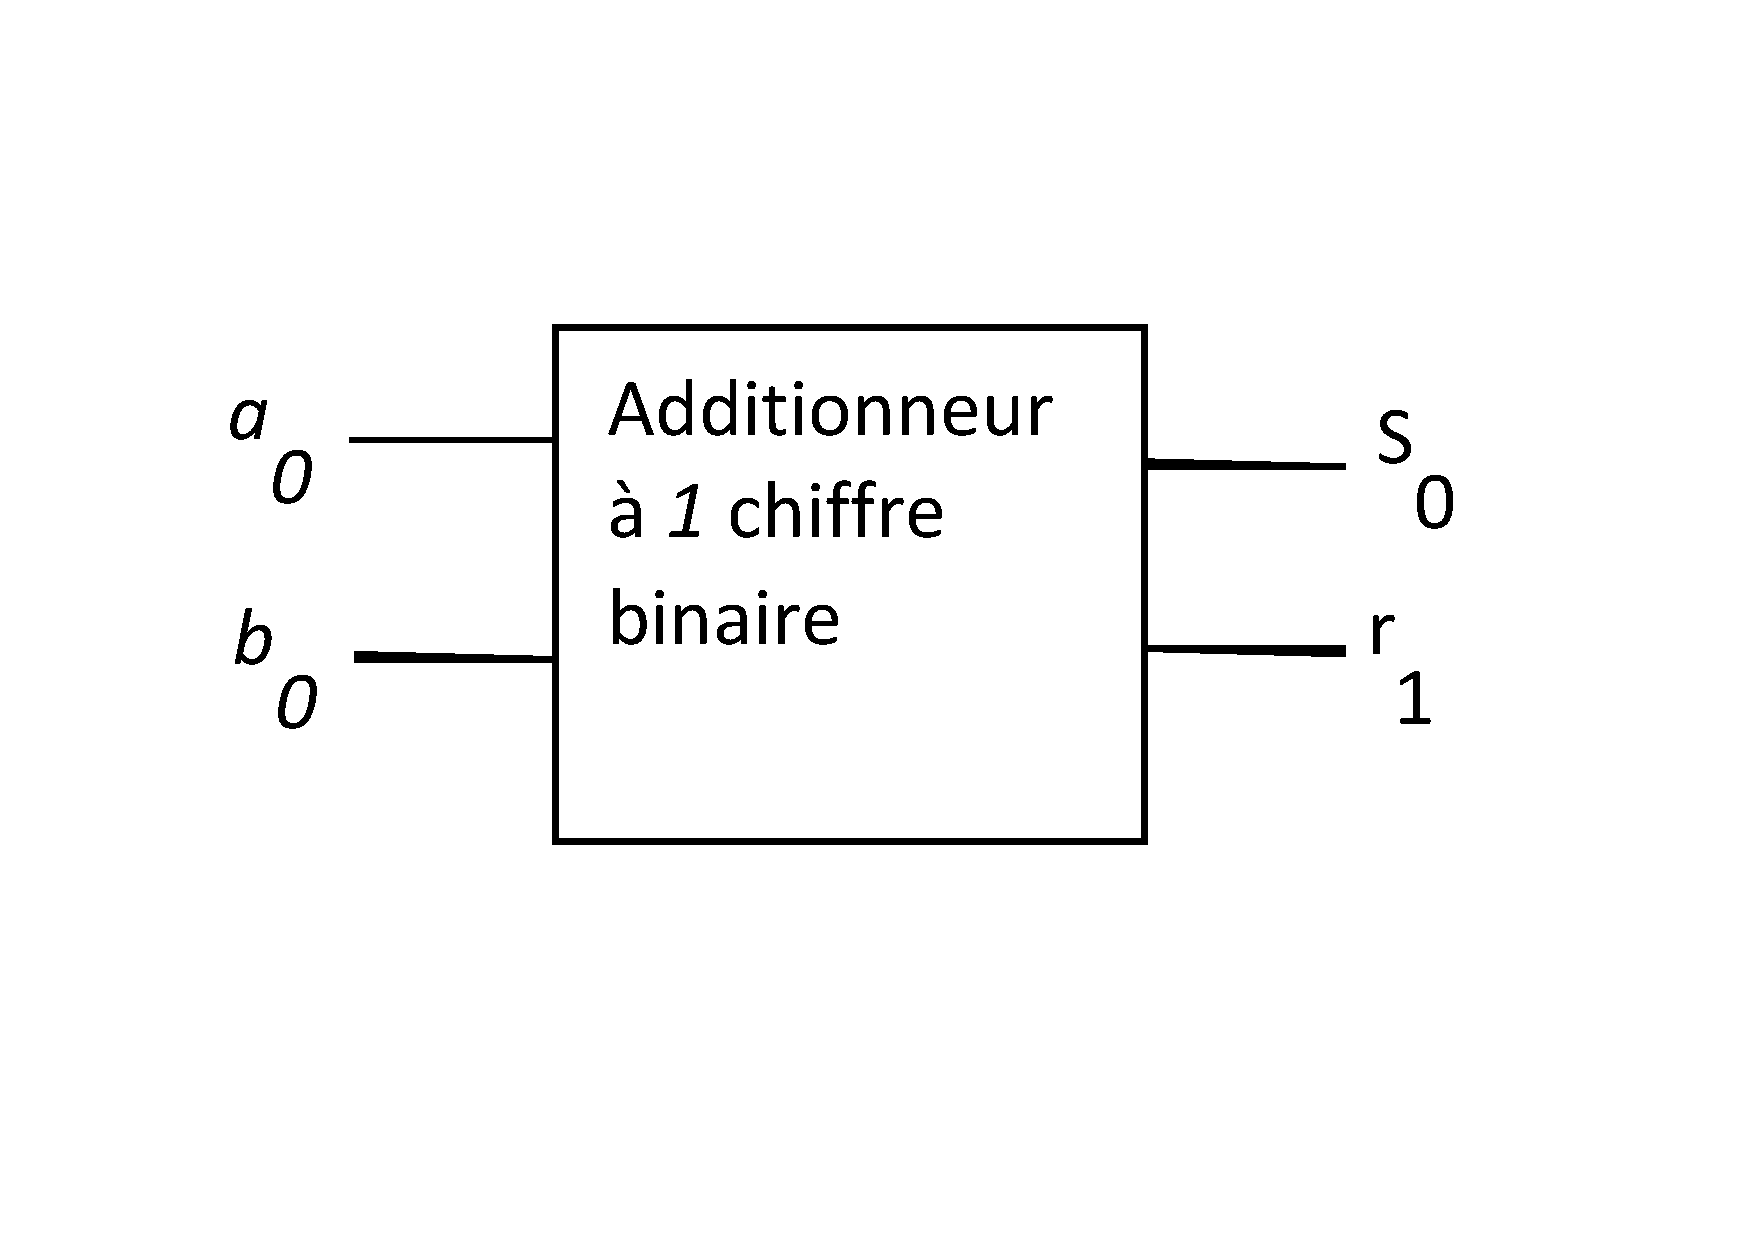
\includegraphics[width=0.8\linewidth]{img/figures04.pdf}
\end{minipage}

La sortie (résultat de l'opération arithmétique d'addition) est un nombre binaire à deux chiffres la somme $s_0$ et la retenue $r_i$ qui réalise l'opération suivante :

$\begin{array}{c c}
 & b_0 \\
+& a_0 \\
\hline
r_1 & s_0
\end{array}$ qui se traduit par $\begin{array}{c c}
 & 0 \\
+& 1 \\
\hline
0 & 1
\end{array}$

\question{Etablir la table de vérité de la somme $s_0$ et la retenue $r_1$ en fonction des entrées $b_0$ et $a_0$.}

\begin{center}
$\begin{array}{|c|c|c|c|}
\hline
b_0 & a_0 & s_0 & r_1 \\
\hline
0   & 0   &     & \\
\hline
0   & 1   &     & \\
\hline
1   & 0   &     & \\
\hline
1   & 1   &     & \\
\hline
\end{array}$
\end{center}

\question{Etablir les équations logiques de la somme $s_0$ (en utilisant un opérateur logique remarquable) et la retenue $r_1$ en fonction des entrées $b_0$ et $a_0$. Vérifier le résultat à l'aide des logiciels de simulation.}

\section{Additionner deux nombres de n bit}

\question{Etablir la table de vérité de la somme $s_1$ (en utilisant un opérateur logique remarquable) et la retenue $r_2$ en fonction des entrées $b_1$, $a_1$ et $r_1$.}

\begin{center}
$\begin{array}{|c|c|c|c|c|}
\hline
b_1 & a_1 & r_1 & s_1 & r_2 \\
\hline
0   & 0 & 0  &  & \\
\hline
0   & 0 & 1  &  & \\
\hline
0   & 1 & 0  &  & \\
\hline
0   & 1 & 1  &  & \\
\hline
1   & 0 & 0  &  & \\
\hline
1   & 0 & 1  &  & \\
\hline
1   & 1 & 0  &  & \\
\hline
1   & 1 & 1  &  & \\
\hline
\end{array}$
\end{center}

\question{Établir les équations logiques de la somme $s_1$ et la retenue $r_2$ en fonction des entrées $b_1$, $a_1$ et $r_1$. Vérifier le résultat à l'aide des logiciels de simulation.}

\question{En déduire les équations logiques de la somme $s_i$ au rang $i$ (en utilisant un opérateur logique remarquable) et la retenue $r_{i+i}$ au rang $i+1$ en fonction des entrées $a_i$, $b_i$ et $r_i$ au rang $i$.}

\question{Tracer le schéma de l'ensemble du système de traitement de l'information.}

\question{Compléter le fichier python afin d'obtenir le même fonctionnement en logique programmée.}

\section{Afficher l'information sur un afficheur 7 segments}

Un afficheur \og 7 segments \fg est constitué de 7 diodes électroluminescentes (LEDs) numérotées de 0 à 6. L'objectif de cette partie est de concevoir un adaptateur qui convertit un nombre binaire pour l'afficher sur un afficheur 7 segments.

\begin{minipage}{0.3\linewidth}
L'adaptateur se présente sous la forme d'un opérateur à 4 entrées binaires $a_3$, $a_2$, $a_1$, $a_0$ et 7 sorties binaires $F_i$ avec $i \in \left[0,6\right]$.
\end{minipage}
\hfill
\begin{minipage}{0.3\linewidth}
 \centering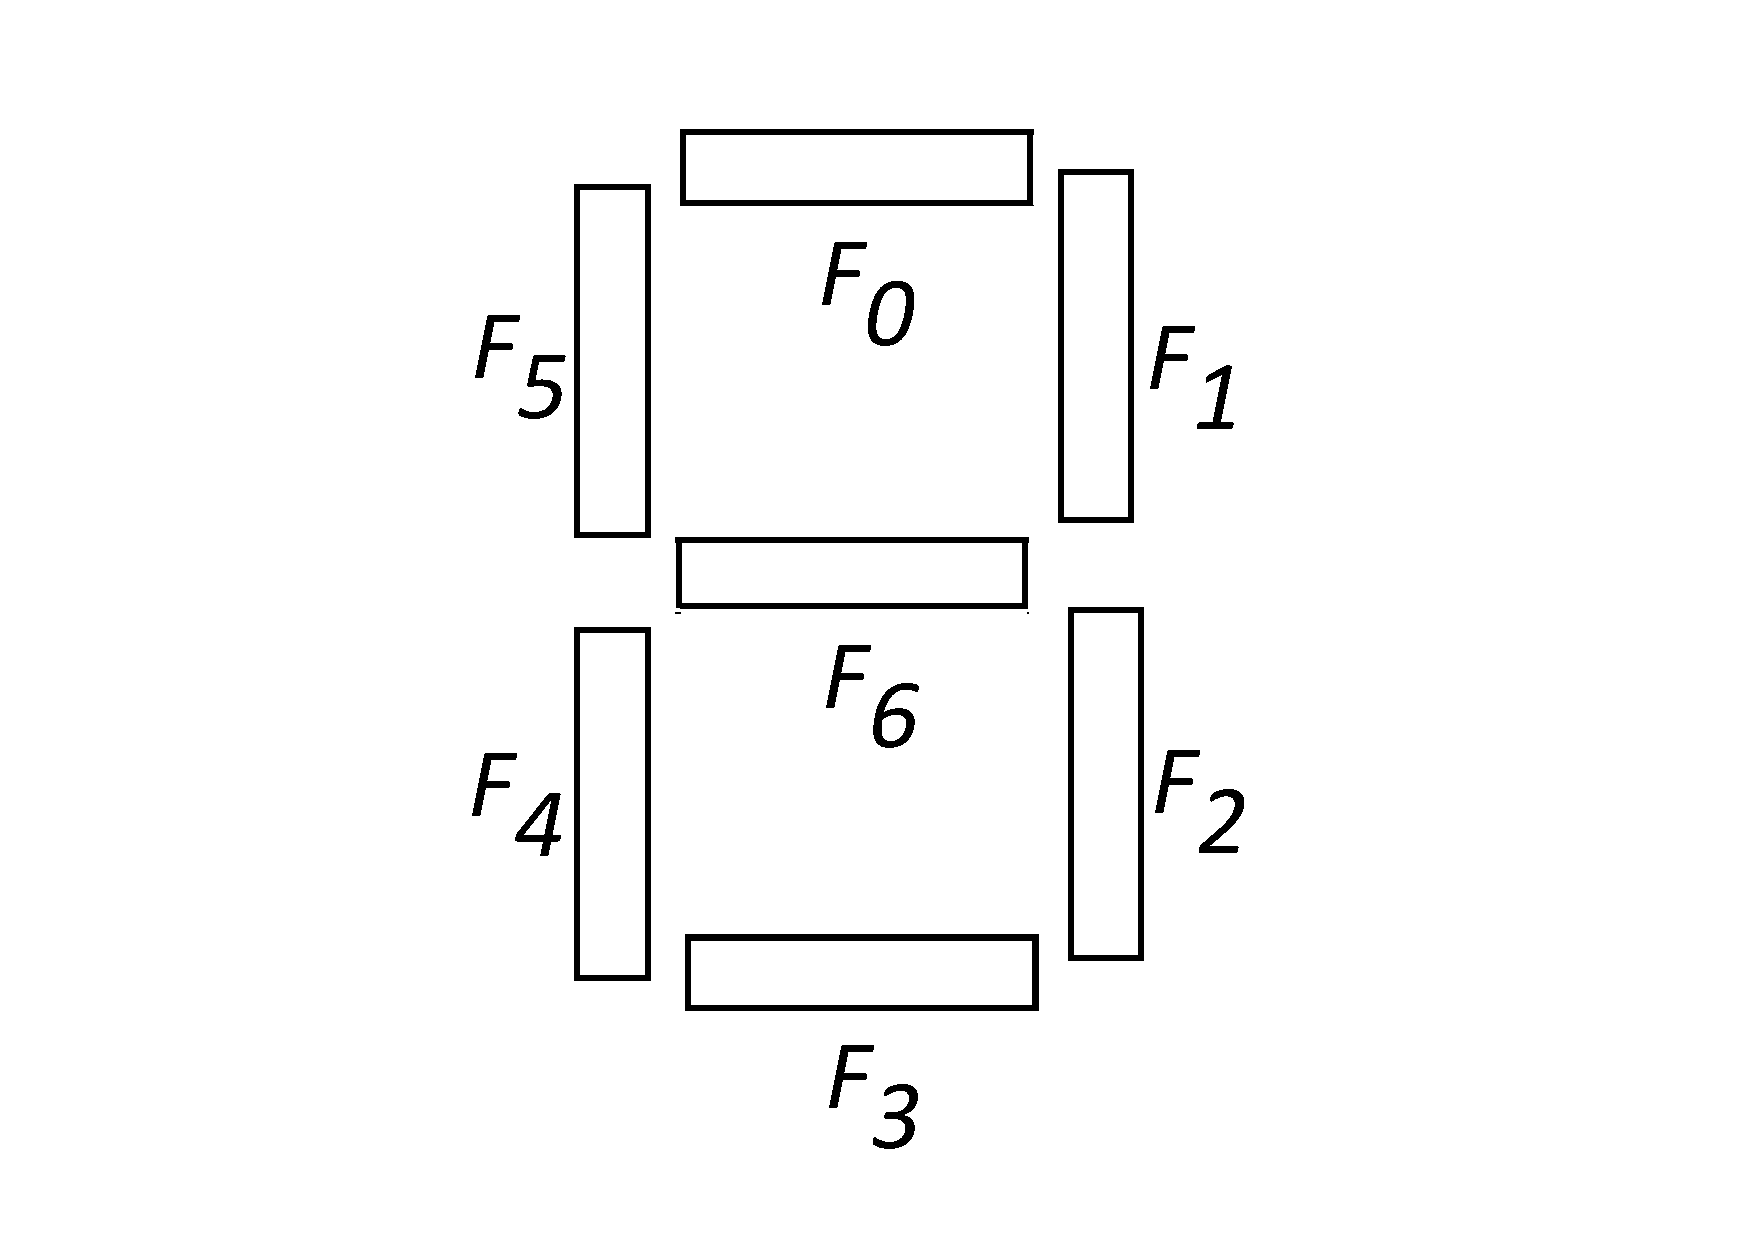
\includegraphics[width=0.8\linewidth]{img/figures02.pdf}
\end{minipage}
\hfill
\begin{minipage}{0.3\linewidth}
 \centering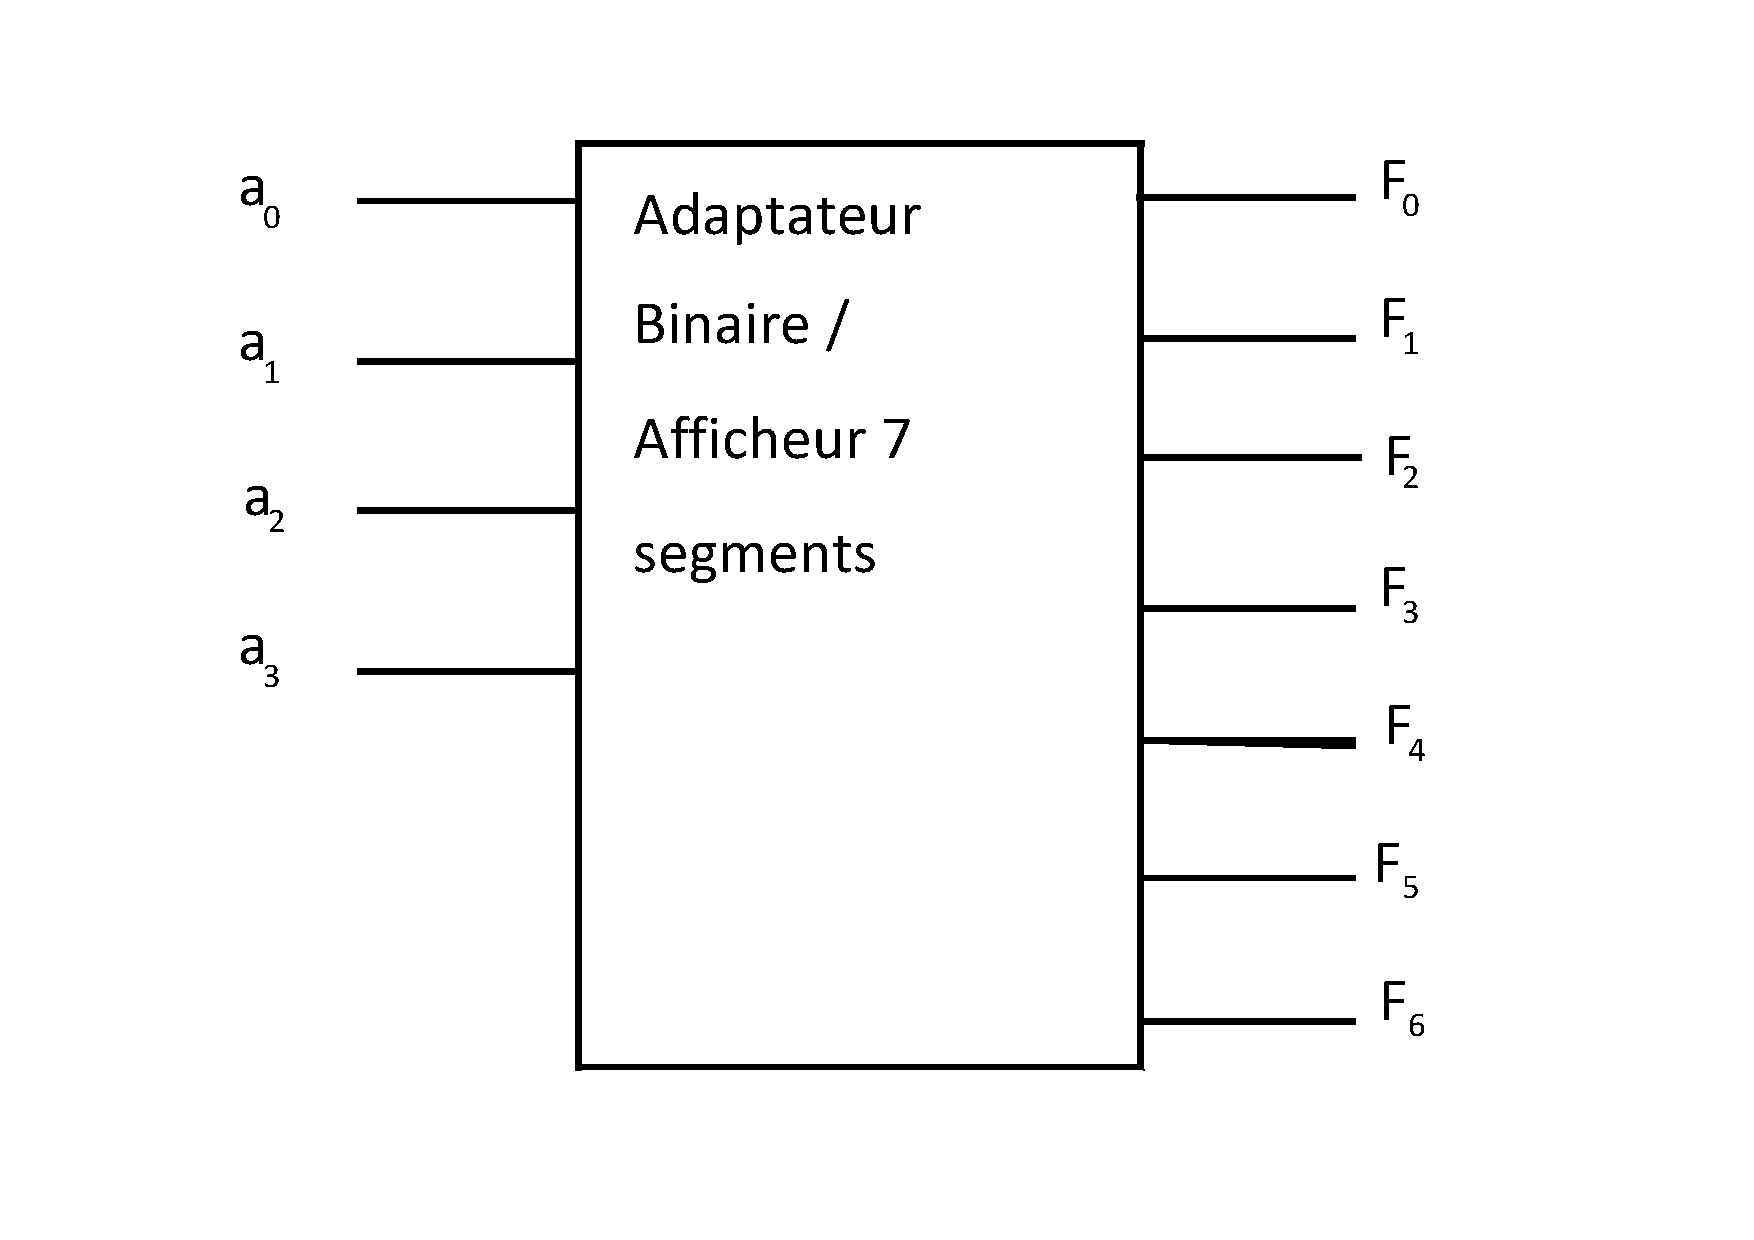
\includegraphics[width=0.8\linewidth]{img/figures03.pdf}
\end{minipage}

\question{Remplir les colonnes $F_i$ de la table de vérité.}

\begin{center}
$\begin{array}{|c|c|c|c||c|c|c|c|c|c|c||c|c|c|c||c|c|c|c|c|c|c|}
\hline
a_3 & a_2 & a_1 & a_0 & F_0 & F_1 & F_2 & F_3 & F_4 & F_5 & F_6 & a_3 & a_2 & a_1 & a_0 & F_0 & F_1 & F_2 & F_3 & F_4 & F_5 & F_6  \\
\hline
0 & 0 & 0 & 0 &  &  &  &  &  &  &  & 1 & 0 & 0 & 0 &  &  &  &  &  &  &  \\
\hline
0 & 0 & 0 & 1 &  &  &  &  &  &  &  & 1 & 0 & 0 & 1 &  &  &  &  &  &  &  \\
\hline
0 & 0 & 1 & 0 &  &  &  &  &  &  &  & 1 & 0 & 1 & 0 &  &  &  &  &  &  &  \\
\hline
0 & 0 & 1 & 1 &  &  &  &  &  &  &  & 1 & 0 & 1 & 1 &  &  &  &  &  &  &  \\
\hline
0 & 1 & 0 & 0 &  &  &  &  &  &  &  & 1 & 1 & 0 & 0 &  &  &  &  &  &  &  \\
\hline
0 & 1 & 0 & 1 &  &  &  &  &  &  &  & 1 & 1 & 0 & 1 &  &  &  &  &  &  &  \\
\hline
0 & 1 & 1 & 0 &  &  &  &  &  &  &  & 1 & 1 & 1 & 0 &  &  &  &  &  &  &  \\
\hline
0 & 1 & 1 & 1 &  &  &  &  &  &  &  & 1 & 1 & 1 & 1 &  &  &  &  &  &  &  \\
\hline
\end{array}$
\end{center}

\question{Etablir l'équation logique de chaque LED $F_i=f_i(a_3,a_2,a_1,a_0)$ de l'afficheur 7 segments à l'aide d'un tableau de Karnaugh.}

\begin{center}
$\begin{array}{|c|c|c|c|c|}
\hline
F_0 & a_1a_0=00 & a_1a_0=01 & a_1a_0=11 & a_1a_0=10 \\
\hline
a_3a_2=00  &    &    &    &    \\
\hline
a_3a_2=01  &    &    &    &    \\
\hline
a_3a_2=11  &    &    &    &    \\
\hline
a_3a_2=10  &    &    &    &    \\
\hline
\end{array}$
\end{center}

\begin{center}
$\begin{array}{|c|c|c|c|c|}
\hline
F_1 & a_1a_0=00 & a_1a_0=01 & a_1a_0=11 & a_1a_0=10 \\
\hline
a_3a_2=00  &    &    &    &    \\
\hline
a_3a_2=01  &    &    &    &    \\
\hline
a_3a_2=11  &    &    &    &    \\
\hline
a_3a_2=10  &    &    &    &    \\
\hline
\end{array}$
\end{center}

\begin{center}
$\begin{array}{|c|c|c|c|c|}
\hline
F_2 & a_1a_0=00 & a_1a_0=01 & a_1a_0=11 & a_1a_0=10 \\
\hline
a_3a_2=00  &    &    &    &    \\
\hline
a_3a_2=01  &    &    &    &    \\
\hline
a_3a_2=11  &    &    &    &    \\
\hline
a_3a_2=10  &    &    &    &    \\
\hline
\end{array}$
\end{center}

\begin{center}
$\begin{array}{|c|c|c|c|c|}
\hline
F_3 & a_1a_0=00 & a_1a_0=01 & a_1a_0=11 & a_1a_0=10 \\
\hline
a_3a_2=00  &    &    &    &    \\
\hline
a_3a_2=01  &    &    &    &    \\
\hline
a_3a_2=11  &    &    &    &    \\
\hline
a_3a_2=10  &    &    &    &    \\
\hline
\end{array}$
\end{center}

\begin{center}
$\begin{array}{|c|c|c|c|c|}
\hline
F_4 & a_1a_0=00 & a_1a_0=01 & a_1a_0=11 & a_1a_0=10 \\
\hline
a_3a_2=00  &    &    &    &    \\
\hline
a_3a_2=01  &    &    &    &    \\
\hline
a_3a_2=11  &    &    &    &    \\
\hline
a_3a_2=10  &    &    &    &    \\
\hline
\end{array}$
\end{center}

\begin{center}
$\begin{array}{|c|c|c|c|c|}
\hline
F_5 & a_1a_0=00 & a_1a_0=01 & a_1a_0=11 & a_1a_0=10 \\
\hline
a_3a_2=00  &    &    &    &    \\
\hline
a_3a_2=01  &    &    &    &    \\
\hline
a_3a_2=11  &    &    &    &    \\
\hline
a_3a_2=10  &    &    &    &    \\
\hline
\end{array}$
\end{center}

\begin{center}
$\begin{array}{|c|c|c|c|c|}
\hline
F_6 & a_1a_0=00 & a_1a_0=01 & a_1a_0=11 & a_1a_0=10 \\
\hline
a_3a_2=00  &    &    &    &    \\
\hline
a_3a_2=01  &    &    &    &    \\
\hline
a_3a_2=11  &    &    &    &    \\
\hline
a_3a_2=10  &    &    &    &    \\
\hline
\end{array}$
\end{center}

\question{Coder à la suite du code python la fonction \verb?f? qui donne la liste $F=[F_0,F_1,F_2,F_3,F_4,F_5,F_6]$ à partir de la liste $a=[a_0,a_1,a_2,a_3]$.}

\clearpage

\ifdef{\public}{\end{document}}{}

\newpage
\setcounter{num_quest}{0}
\pagestyle{correction}

\section{Correction}

\question{Etablir la table de vérité de la somme $s_0$ et la retenue $r_1$ en fonction des entrées $b_0$ et $a_0$.}

\begin{center}
$\begin{array}{|c|c|c|c|}
\hline
b_0 & a_0 & s_0 & r_1 \\
\hline
0   & 0   &  0  & 0 \\
\hline
0   & 1   &  1  & 0 \\
\hline
1   & 0   &  1  & 0 \\
\hline
1   & 1   &  0  & 1 \\
\hline
\end{array}$
\end{center}

\question{Etablir les équations logiques de la somme $s_0$ (en utilisant un opérateur logique remarquable) et la retenue $r_1$ en fonction des entrées $b_0$ et $a_0$. Vérifier le résultat à l'aide des logiciels de simulation.}

$s_0=a_0\oplus b_0$, $r_1=a_0.b_0$

\question{Etablir la table de vérité de la somme $s_1$ (en utilisant un opérateur logique remarquable) et la retenue $r_2$ en fonction des entrées $b_1$, $a_1$ et $r_1$.}

\begin{center}
$\begin{array}{|c|c|c|c|c|}
\hline
b_1 & a_1 & r_1 & s_1 & r_2 \\
\hline
0   & 0 & 0  & 0 & 0 \\
\hline
0   & 0 & 1  & 1 & 0 \\
\hline
0   & 1 & 0  & 1 & 0 \\
\hline
0   & 1 & 1  & 0 & 1 \\
\hline
1   & 0 & 0  & 1 & 0 \\
\hline
1   & 0 & 1  & 0 & 1 \\
\hline
1   & 1 & 0  & 0 & 1 \\
\hline
1   & 1 & 1  & 1 & 1 \\
\hline
\end{array}$
\end{center}

\question{Établir les équations logiques de la somme $s_1$ et la retenue $r_2$ en fonction des entrées $b_1$, $a_1$ et $r_1$. Vérifier le résultat à l'aide des logiciels de simulation.}

$s_1=a_1\oplus b_1\oplus r_1$, $r_2=a_1.b_1+b_1.r_1+r_1.a_1$\\

\question{En déduire les équations logiques de la somme $s_i$ au rang $i$ (en utilisant un opérateur logique remarquable) et la retenue $r_{i+i}$ au rang $i+1$ en fonction des entrées $a_i$, $b_i$ et $r_i$ au rang $i$.}

$s_i=a_i\oplus b_i\oplus r_i$, $r_{i+1}=a_i.b_i+b_i.r_i+r_i.a_i$

\question{Tracer le schéma de l'ensemble du système de traitement de l'information.}

\begin{center}
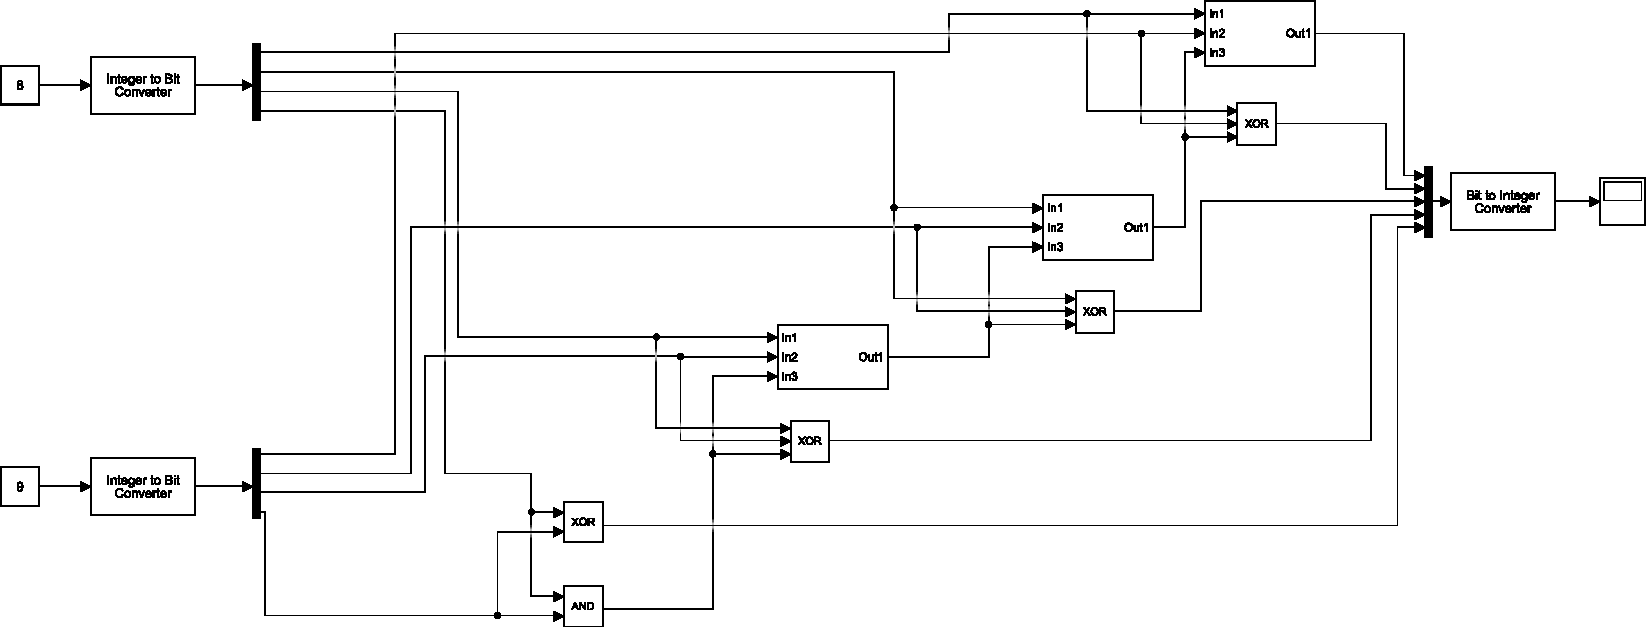
\includegraphics[width=0.8\linewidth]{img/calculatrice_1}\\
Décomposition des sous-blocs\\
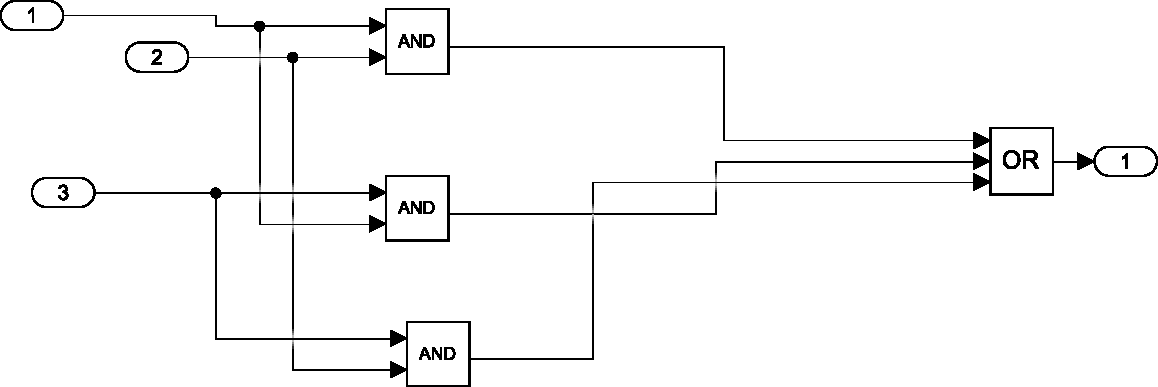
\includegraphics[width=0.5\linewidth]{img/calculatrice_2}
\end{center}

\question{Compléter le fichier python afin d'obtenir le même fonctionnement en logique programmée.}

Le code est disponible \href{https://github.com/Costadoat/S10/raw/master/TP01\%20Fonctions\%20combinatoires/Code/Calculatrice.py}{ici}.

\question{Remplir les colonnes $F_i$ de la table de vérité.}

\begin{center}
$\begin{array}{|c|c|c|c||c|c|c|c|c|c|c||c|c|c|c||c|c|c|c|c|c|c|}
\hline
a_3 & a_2 & a_1 & a_0 & F_0 & F_1 & F_2 & F_3 & F_4 & F_5 & F_6 & a_3 & a_2 & a_1 & a_0 & F_0 & F_1 & F_2 & F_3 & F_4 & F_5 & F_6  \\
\hline
0 & 0 & 0 & 0 & 1 & 1 & 1 & 1 & 1 & 1 & 0 & 1 & 0 & 0 & 0 & 1 & 1 & 1 & 1 & 1 & 1 & 1 \\
\hline
0 & 0 & 0 & 1 & 0 & 1 & 1 & 0 & 0 & 0 & 0 & 1 & 0 & 0 & 1 & 1 & 1 & 1 & 1 & 0 & 1 & 1 \\
\hline
0 & 0 & 1 & 0 & 1 & 1 & 0 & 1 & 1 & 0 & 1 & 1 & 0 & 1 & 0 & 1 & 1 & 1 & 0 & 1 & 1 & 1 \\
\hline
0 & 0 & 1 & 1 & 1 & 1 & 1 & 1 & 0 & 0 & 1 & 1 & 0 & 1 & 1 & 0 & 0 & 1 & 1 & 1 & 1 & 1 \\
\hline
0 & 1 & 0 & 0 & 0 & 1 & 1 & 0 & 0 & 1 & 1 & 1 & 1 & 0 & 0 & 1 & 0 & 0 & 1 & 1 & 1 & 0 \\
\hline
0 & 1 & 0 & 1 & 1 & 0 & 1 & 1 & 0 & 1 & 1 & 1 & 1 & 0 & 1 & 0 & 1 & 1 & 1 & 1 & 0 & 1 \\
\hline
0 & 1 & 1 & 0 & 1 & 0 & 1 & 1 & 1 & 1 & 1 & 1 & 1 & 1 & 0 & 1 & 0 & 0 & 1 & 1 & 1 & 1 \\
\hline
0 & 1 & 1 & 1 & 1 & 1 & 1 & 0 & 0 & 0 & 0 & 1 & 1 & 1 & 1 & 1 & 0 & 0 & 0 & 1 & 1 & 1 \\
\hline
\end{array}$
\end{center}

\question{Etablir l'équation logique de chaque LED $F_i=f_i(a_3,a_2,a_1,a_0)$ de l'afficheur 7 segments à l'aide d'un tableau de Karnaugh.}

\begin{center}
$\begin{array}{|c|c|c|c|c|}
\hline
F_0 & a_1a_0=00 & a_1a_0=01 & a_1a_0=11 & a_1a_0=10 \\
\hline
a_3a_2=00  &  1  &  0  & 1   &  1  \\
\hline
a_3a_2=01  &  0  &   1 &  1  &  1  \\
\hline
a_3a_2=11  &  1  &  0  &  1  &  1  \\
\hline
a_3a_2=10  &  1  & 1   &  0  &  1  \\
\hline
\end{array}$
\end{center}

\begin{center}
$\begin{array}{|c|c|c|c|c|}
\hline
F_1 & a_1a_0=00 & a_1a_0=01 & a_1a_0=11 & a_1a_0=10 \\
\hline
a_3a_2=00  & 1   &  1  &  1  &  1  \\
\hline
a_3a_2=01  &  1  &  0  & 1   & 0   \\
\hline
a_3a_2=11  &   1 & 0   & 1   & 1   \\
\hline
a_3a_2=10  &  1  & 1   & 0   & 1   \\
\hline
\end{array}$
\end{center}

\begin{center}
$\begin{array}{|c|c|c|c|c|}
\hline
F_2 & a_1a_0=00 & a_1a_0=01 & a_1a_0=11 & a_1a_0=10 \\
\hline
a_3a_2=00  &  1  & 1   & 1   &  0  \\
\hline
a_3a_2=01  &  1  &  1  &  1  &  1  \\
\hline
a_3a_2=11  &  0  & 1   & 0   &  0  \\
\hline
a_3a_2=10  &  1  &  1  &  1  & 1   \\
\hline
\end{array}$
\end{center}

\begin{center}
$\begin{array}{|c|c|c|c|c|}
\hline
F_3 & a_1a_0=00 & a_1a_0=01 & a_1a_0=11 & a_1a_0=10 \\
\hline
a_3a_2=00  &  1  &  0  &  1  &   1 \\
\hline
a_3a_2=01  &  0  &  1  &  0  &  1  \\
\hline
a_3a_2=11  &  1  &  1  &  0  &  1  \\
\hline
a_3a_2=10  &  1  & 1   &  1  & 0   \\
\hline
\end{array}$
\end{center}

\begin{center}
$\begin{array}{|c|c|c|c|c|}
\hline
F_4 & a_1a_0=00 & a_1a_0=01 & a_1a_0=11 & a_1a_0=10 \\
\hline
a_3a_2=00  &  1  &  0  &  0  &  1  \\
\hline
a_3a_2=01  &   0 &  0  &  0  &  1  \\
\hline
a_3a_2=11  &  1  &  1  &  1  &  1  \\
\hline
a_3a_2=10  & 1   &  0  &  1  & 1   \\
\hline
\end{array}$
\end{center}

\begin{center}
$\begin{array}{|c|c|c|c|c|}
\hline
F_5 & a_1a_0=00 & a_1a_0=01 & a_1a_0=11 & a_1a_0=10 \\
\hline
a_3a_2=00  & 1   &  0  &  0  &  0  \\
\hline
a_3a_2=01  &  1  &  1  &  0  &  1  \\
\hline
a_3a_2=11  &  1  &  0  &  1  &  1  \\
\hline
a_3a_2=10  &  1  &  1  & 1   &  1  \\
\hline
\end{array}$
\end{center}

\begin{center}
$\begin{array}{|c|c|c|c|c|}
\hline
F_6 & a_1a_0=00 & a_1a_0=01 & a_1a_0=11 & a_1a_0=10 \\
\hline
a_3a_2=00  & 0   &  0  &  1  &  1  \\
\hline
a_3a_2=01  &  1  &  1  &  0  & 1   \\
\hline
a_3a_2=11  &  0  &  1  &  1  & 1   \\
\hline
a_3a_2=10  &  1  &  1  &  1  & 1   \\
\hline
\end{array}$
\end{center}


$F_0=\overline{a_3}.a_1+a_2.a_1+\overline{a_2}.\overline{a_0}+a_3.\overline{a_0}+a_3.\overline{a_2}.\overline{a_1}+\overline{a_3}.a_2.a_0$

$F_1=\overline{a_1}.\overline{a_0}+\overline{a_3}.\overline{a_2}+a_2.a_1.a_0+a_3.\overline{a_0}+\overline{a_2}.\overline{a_1}$

$F_2=\overline{a_3}.\overline{a_1}+\overline{a_3}.a_0+\overline{a_1}.a_0+a_3.\overline{a_2}+\overline{a_3}.a_2$

$F_3=a_3.\overline{a_1}+\overline{a_3}.\overline{a_2}.\overline{a_0}+\overline{a_3}.\overline{a_2}.a_1+a_2.\overline{a_1}.a_0+a_2.a_1.\overline{a_0}+a_3.\overline{a_2}.a_0$

$F_4=a_3.a_2+a_1.\overline{a_0}+a_3.a_1+\overline{a_2}.\overline{a_0}$

$F_5=\overline{a_1}.\overline{a_0}+a_3.a_1+a_2.\overline{a_0}+\overline{a_3}.a_2.\overline{a_1}+a_3.\overline{a_2}$

$F_6=a_1.\overline{a_0}+a_3.\overline{a_2}+a_3.a_0+\overline{a_2}.a_1+\overline{a_3}.a_2.\overline{a_1}$

\question{Coder à la suite du code python la fonction \verb?f? qui donne la liste $F=[F_0,F_1,F_2,F_3,F_4,F_5,F_6]$ à partir de la liste $a=[a_0,a_1,a_2,a_3]$.}

Le code est disponible \href{https://github.com/Costadoat/S10/raw/master/TP01\%20Fonctions\%20combinatoires/Code/Calculatrice.py}{ici}.

\begin{verbatim}
def f(a):
    fr=[]
    fr.append(not a[3] and a[1] or a[2] and a[1] or not a[2] and not a[0]
    		or a[3] and not a[0] or a[3]and not a[2] and not a[1]
    		or not a[3]and a[2] and a[0])
    fr.append(not a[1]and not a[0] or not a[3]and not a[2]or a[2]and a[1]and a[0]
    		or a[3] and not a[0]or not a[2]and not a[1])
    fr.append(not a[3]and not a[1]or not a[3]and a[0] or not a[1] and a[0]
    		or a[3] and not a[2] or not a[3]and a[2])
    fr.append(a[3]and not a[1] or not a[3]and not a[2] and not a[0]
    		or not a[3]and not a[2]and a[1]or a[2]and not a[1]and a[0]
    		or a[2]and a[1]and not a[0]or a[3]and not a[2]and a[0])
    fr.append(a[3]and a[2]or a[1]and not a[0] or a[3]and a[1]
    		or not a[2]and not a[0])
    fr.append(not a[1]and not a[0]or a[3]and a[1]or a[2]and not a[0]
    		or not a[3]and a[2]and not a[1]or a[3]and not a[2])
    fr.append(a[1]and not a[0]or a[3]and not a[2]or a[3]and a[0]
    		or not a[2]and a[1]or not a[3]and a[2]and not a[1])
    return fr
\end{verbatim}
    
\end{document}
